% This is "sig-alternate.tex" V2.1 April 2013
% This file should be compiled with V2.5 of "sig-alternate.cls" May 2012
%
% This example file demonstrates the use of the 'sig-alternate.cls'
% V2.5 LaTeX2e document class file. It is for those submitting
% articles to ACM Conference Proceedings WHO DO NOT WISH TO
% STRICTLY ADHERE TO THE SIGS (PUBS-BOARD-ENDORSED) STYLE.
% The 'sig-alternate.cls' file will produce a similar-looking,
% albeit, 'tighter' paper resulting in, invariably, fewer pages.
%
% ----------------------------------------------------------------------------------------------------------------
% This .tex file (and associated .cls V2.5) produces:
%       1) The Permission Statement
%       2) The Conference (location) Info information
%       3) The Copyright Line with ACM data
%       4) NO page numbers
%
% as against the acm_proc_article-sp.cls file which
% DOES NOT produce 1) thru' 3) above.
%
% Using 'sig-alternate.cls' you have control, however, from within
% the source .tex file, over both the CopyrightYear
% (defaulted to 200X) and the ACM Copyright Data
% (defaulted to X-XXXXX-XX-X/XX/XX).
% e.g.
% \CopyrightYear{2007} will cause 2007 to appear in the copyright line.
% \crdata{0-12345-67-8/90/12} will cause 0-12345-67-8/90/12 to appear in the copyright line.
%
% ---------------------------------------------------------------------------------------------------------------
% This .tex source is an example which *does* use
% the .bib file (from which the .bbl file % is produced).
% REMEMBER HOWEVER: After having produced the .bbl file,
% and prior to final submission, you *NEED* to 'insert'
% your .bbl file into your source .tex file so as to provide
% ONE 'self-contained' source file.
%
% ================= IF YOU HAVE QUESTIONS =======================
% Questions regarding the SIGS styles, SIGS policies and
% procedures, Conferences etc. should be sent to
% Adrienne Griscti (griscti@acm.org)
%
% Technical questions _only_ to
% Gerald Murray (murray@hq.acm.org)
% ===============================================================
%
% For tracking purposes - this is V2.0 - May 2012



\documentclass{sig-alternate-05-2015}

\begin{document}

% Copyright
\setcopyright{acmcopyright}
%\setcopyright{acmlicensed}
%\setcopyright{rightsretained}
%\setcopyright{usgov}
%\setcopyright{usgovmixed}
%\setcopyright{cagov}
%\setcopyright{cagovmixed}


% DOI
\doi{10.475/123_4}

% ISBN
\isbn{123-4567-24-567/08/06}

%Conference
\conferenceinfo{PLDI '13}{June 16--19, 2013, Seattle, WA, USA}

\acmPrice{\$15.00}

%
% --- Author Metadata here ---
\conferenceinfo{WOODSTOCK}{'97 El Paso, Texas USA}
%\CopyrightYear{2007} % Allows default copyright year (20XX) to be over-ridden - IF NEED BE.
%\crdata{0-12345-67-8/90/01}  % Allows default copyright data (0-89791-88-6/97/05) to be over-ridden - IF NEED BE.
% --- End of Author Metadata ---

\title{ Mining HIV Trends in Social Media Data}
%
% You need the command \numberofauthors to handle the 'placement
% and alignment' of the authors beneath the title.
%
% For aesthetic reasons, we recommend 'three authors at a time'
% i.e. three 'name/affiliation blocks' be placed beneath the title.
%
% NOTE: You are NOT restricted in how many 'rows' of
% "name/affiliations" may appear. We just ask that you restrict
% the number of 'columns' to three.
%
% Because of the available 'opening page real-estate'
% we ask you to refrain from putting more than six authors
% (two rows with three columns) beneath the article title.
% More than six makes the first-page appear very cluttered indeed.
%
% Use the \alignauthor commands to handle the names
% and affiliations for an 'aesthetic maximum' of six authors.
% Add names, affiliations, addresses for
% the seventh etc. author(s) as the argument for the
% \additionalauthors command.
% These 'additional authors' will be output/set for you
% without further effort on your part as the last section in
% the body of your article BEFORE References or any Appendices.

\numberofauthors{2} %  in this sample file, there are a *total*
% of EIGHT authors. SIX appear on the 'first-page' (for formatting
% reasons) and the remaining two appear in the \additionalauthors section.
%
\author{
% You can go ahead and credit any number of authors here,
% e.g. one 'row of three' or two rows (consisting of one row of three
% and a second row of one, two or three).
%
% The command \alignauthor (no curly braces needed) should
% precede each author name, affiliation/snail-mail address and
% e-mail address. Additionally, tag each line of
% affiliation/address with \affaddr, and tag the
% e-mail address with \email.
%
% 1st. author
\alignauthor
Patrick Breen\\
       \affaddr{The Institute of Bioinformatics}\\
       \affaddr{The University of Georgia}\\
       \affaddr{Athens, Georgia}\\
       \email{pbreen@uga.edu}
% 2nd. author
\alignauthor
Shannon Quinn\titlenote{Corresponding author.}\\
       \affaddr{Institute of Computer Science}\\
       \affaddr{University of Georgia}\\
       \affaddr{Athens, Georgia}\\
       \email{squinn@cs.uga.edu}
}



\maketitle
\begin{abstract}

Pre-Exposure Prophylaxis (PrEP) is a recently developed therapy for the prevention of Human Immunodeficiency Virus (HIV). The treatment is available as a pill named Truvada and is taken once a day for as much as 99\% protection from infection when exposed to HIV. While medically effective, PrEP suffers from high drug costs, HIV-related social stigma, and under-informed health providers and patients. This paper contributes a data mining and machine learning strategy that monitors Twitter social media data to determine HIV and PrEP discussion trends. Our results show that we can identify PrEP and HIV discussion dynamics over time, and positive and negative PrEP-related tweets. These results can be used by public health professionals to inform and protect at-risk individuals from HIV. 

%These methods may also be useful to identify and preempt HIV outbreaks before they reach epidemic levels.

\end{abstract}


%
% The code below should be generated by the tool at
% http://dl.acm.org/ccs.cfm
% Please copy and paste the code instead of the example below. 
%
% TODO: this section
\begin{CCSXML}

\end{CCSXML}


%
% End generated code
%

%
%  Use this command to print the description
%
\printccsdesc

% We no longer use \terms command
%\terms{Theory}

\keywords{ Social Media, Topic Modelling, Document Embedding}

\section{Introduction}
Example citation (needed right now to compile):\cite{Lamport:LaTeX}

Introduce and literature review of:
1) PrEP, HIV, Twitter

 - social impact issues, efficacy, adherence issues, other STDs, Austin (Scott County) Indiana Outbreak as example
 
 - High cost of actual drug medication, and unclear health insurance situation.
 
 - Many health providers do not know about drug.
 
 - specifically other papers that did mining Twitter for HIV
 
 - Here is a paper that did twitter data mining for flu prediction:
 
 %http://snap.stanford.edu/soma2010/papers/soma2010_16.pdf
 
 Talk about how it's harder to get feedback/ account for HIV infections compared with CDC baseline data for flu. Talk about twitter-specifc issues such as bots and slang.


2) Word2Vec, Doc2Vec

 - theory and application examples

3) Dynamic Topic models, Latent Dirichlet allocation

- theory and application examples

\section{Results}



We sought to determine trends in HIV and PrEP discourse on twitter, to inform and coordinate public health efforts aiming to promote PrEP adoption and adherence for at-risk individuals. We collected 624,569 tweets containing at least one of the following words 'HIV', 'AIDS', 'truvada', 'prophylaxis', 'imtesting', 'PrEP' from Twitter's streaming API. The tweets were restricted to English language, and the collection dates spanned from the 47th week of 2015 to the 14th week of 2016. The tweets were and cleaned of exotic characters.

We excluded tweets that did not originate in contiguous United States time zones. A subset of the tweets we collected had geolocation data available. We found that tweets were largely concentrated on US and Canadian metro areas (Figure 1).


\begin{figure}
\centering
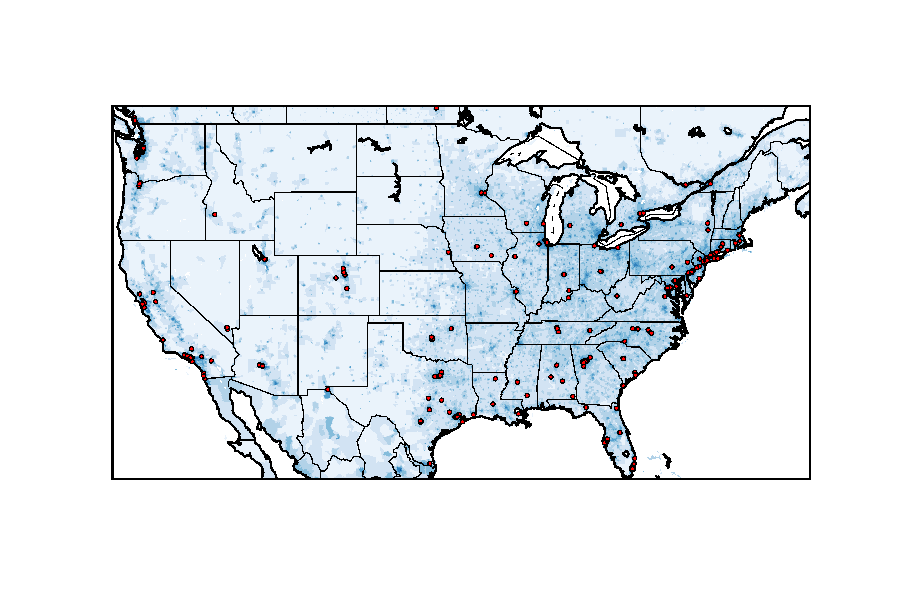
\includegraphics[height=2.5in, width=3.5in]{map}
\caption{Plot of geolocated tweets.}
\end{figure}

\subsection{Word and Document Similarity}

The first analysis that we performed sought to identify certain keywords, hashtags, tweets and users, that were discussed in HIV and PrEP related contexts. Word2Vec and the related method, Paragraph2Vec are unsupervised machine learning methods that have performed well at embedding natural language in a semantic vector space. In our analysis, Word2Vec allows us to determine semantically similar words to a query word, while Paragraph2Vec allows us to determine similar tweets, users and hashtags to a query hashtag.

We trained a Word2Vec model, and queried for the top 10 word-vectors related to the term PrEP (Table 1). We found several HIV related events, WorldAIDSDay, HLM2016AIDS, ICASA2015, as well as the PrEP drug Truvada, and the term HIV. In addition, we found the acronym ART which refers to Anti-Retroviral Therapy. DoingIt, and OneConversation, are ongoing efforts led by the Center for Disease Control (CDC) to spread awareness and reduce the spread of HIV. NBHAAD is an organization that is committed to increasing awareness for HIV within the Black community (TODO: look up if there is some special connection between HIV and Black community). Nancy Reagan, who died in early 2016, was mentioned in conjunction with her efforts to combat HIV in the 1980's. Together these results show us a high-level view of the important components of the national PrEP conversation on Twitter.

% table 1 - w2v PrEP
\begin{table}
\centering
\caption{Cosine Similarity to word-vector 'PrEP'}
\begin{tabular}{|l|c|} \hline
Related Word & Cosine Similarity to 'PrEP'\\ \hline
truvada & 0.796666\\ \hline
DoingIt & 0.738141\\ \hline
WorldAIDSDay & 0.720910\\ \hline
NancyReagan & 0.717667\\ \hline
NBHAAD & 0.705061\\ \hline
ART & 0.704300\\ \hline
HLM2016AIDS & 0.698698\\ \hline
ICASA2015 & 0.693117\\ \hline
HIV & 0.692860\\ \hline
OneConversation & 0.688427\\ \hline
\hline\end{tabular}
\end{table}

Doc2Vec allows us to identify the top users, tweets, and hashtags associated with \#prep. Note that on Twitter, hashtags are not case sensitive. Querying for the top 10 document-level entities associated with \#prep, we again see several PrEP and HIV related hashtags including \#hiv, \#hivprevention, \#truvada, and \#whereisprep. We also see a LGBT-related hashtag, \#lgbtmedia16, which indicates a distinct awareness of PrEP in the Gay community. This may reflect the known levels of HIV transmission in gay men (TODO: cite something here).

Interestingly, we also found 3 tweets and 1 user in the top 10 doc2vec results for \#prep. Tweet 702179860983189504 has content spreading HIV prevention awareness: "\#StoneColdVideoTODAY if You see this 13 symptoms. Do HIV Test Immediately. Must Read". Conversely tweet 708519265540907010 has content that calls into doubt the usefulness of PrEP: "Checkout why PrEP is hurting the cause \& \#JoinTheConversation \#LGBTQIA". User 711275699529764864 is a twitter spam bot with no particular connection to PrEP. Together the Doc2Vec results show that we can monitor and identify PrEP-related hashtags and tweets. The most PrEP related tweets, the content of the above tweets were popular on twitter over the period of data that we collected. When they were retweeted, doc2vec weighted them more highly similar to \#prep. Thus with this method we demonstrate a way to identify and monitor the most viral tweets related to PrEP. As the discussion changes, public health professionals can use this information to quickly identify the most important viral sentiment in the online PrEP conversation.

% table 2 - d2v PrEP
\begin{table}
\centering
\caption{Cosine Similarity to doc-vector '\#PrEP'}
\begin{tabular}{|l|c|} \hline
Related Hashtag/Tweet & Cosine Similarity to '\#PrEP'\\ \hline
\#lgbtmedia16 & 0.739128\\ \hline
\#hiv & 	0.727602 \\ \hline
\#whereisprep & 0.707165 \\ \hline
\#truvada & 0.696113 \\ \hline
\#hivprevention & 0.636068 \\ \hline
tweet-702179860983189504 & 0.630055\\ \hline
user-711275699529764864 & 0.629254\\ \hline
tweet-708519265540907010 & 0.628778 \\ \hline
tweet-712032637024653313 & 0.628646 \\ \hline
\#harrogatehour & 0.628547 \\ \hline
\hline\end{tabular}
\end{table}

Finally we wanted to visualize the relative similarities of these PrEP-related keywords in a low dimensional space. We took several keywords that we had identified in our PrEP related queries, along with other HIV-prevention related terms, and visualised their word-vectors in 2 dimensions using tSNE (Figure 2)(TODO: citation for tSNE.).

We several trends. Notably the pharmaceutical based HIV therapies all cluster together (ART, PrEP, truvada), the AIDS awareness events cluster together (WorldAIDSDay, NBHAAD) and so do the sexually transmitted disease keywords (HIV, AIDS, STD). These results may provide another mechanism for researchers to visualize and identify relevant trends in PrEP-related keywords.

% figure 3
\begin{figure*}
\centering
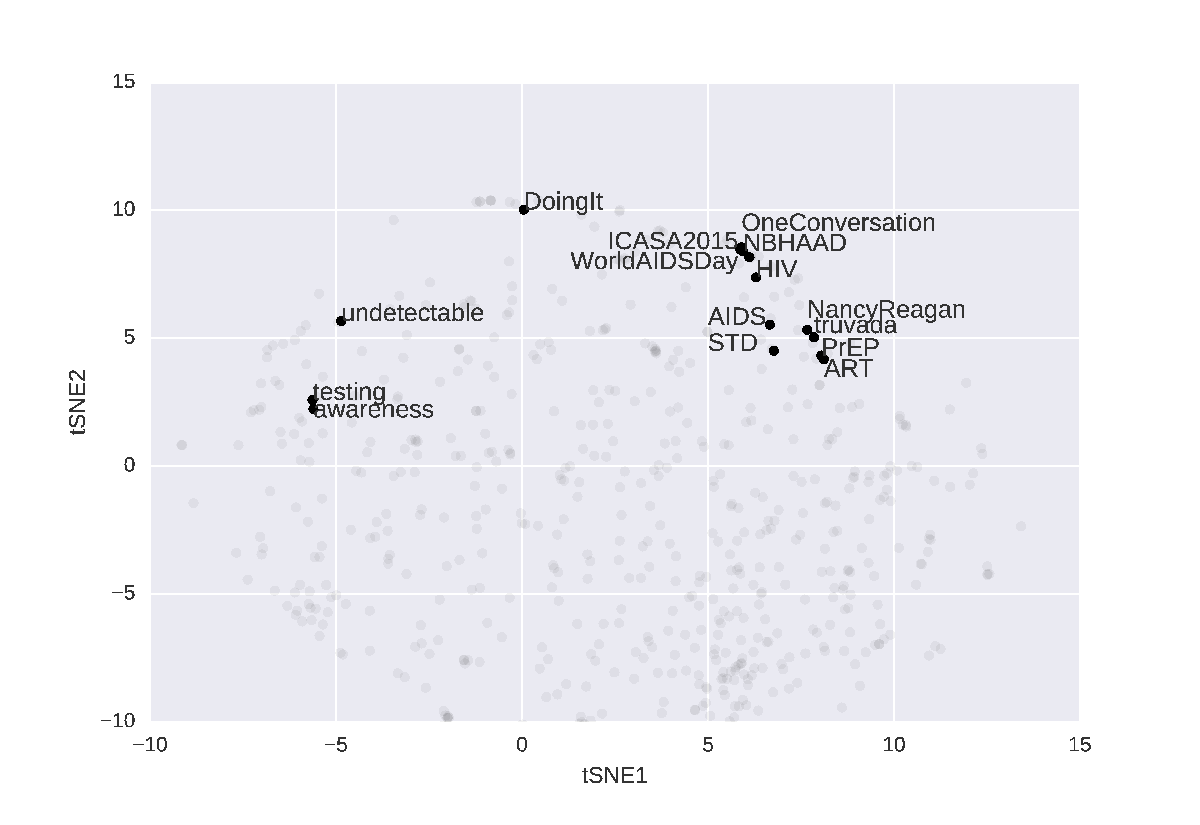
\includegraphics[height=4in, width=6in]{tSNE_word}
\caption{tSNE plot of relevant word-vectors}
\end{figure*}

\subsection{Time Domain}

Next we sought to identify some temporal trends in PrEP related trends. We used Dynamic Topic Modelling (DTM) to identify how certain topics change over time. In DTM, documents are grouped in several corpuses that represent successive points in time. Latent Dirichlet Analysis (LDA) is then performed on each corpus, to extract a topic distribution. The posterior topic distribution from time $t_n$ is used as the prior for time $t_{n+1}$. This lets the model determine a topic model for each time point that is dependent both on the set of tweets from that time point, and on the time point's document distribution. We specified 10 topics and used each week's worth of tweets, over a 30 week period from the 47th week of 2015 to the 14th week of 2016, as our time points.

We identified two topics that showed relevant trends. In topic 5 we see that the keyword 'PrEP' increases over time, while 'prevention', 'drug' and 'risk' remain constant (Figure 3). The term 'pill', also from topic 5, declines overtime. These dynamics may indicate that PrEP discussion is becoming more prevalent. Other HIV prevention related words such as 'pill', 'prevention' and 'drug' which serve as a form of negative controls. They are related to PrEP semantically, and are thus in the same topic. Yet the fact that they are not increasing, shows us that the increase in PrEP discussion is PrEP-specific.

However, it is hard to tell from these data though, whether the increased level of PrEP discussion is leading to increased levels of informed patients, medical providers, and adherence. It is possible that stigma, and misinformation is leading to greater levels of PrEP discussion on twitter. We will get more specific, granular understanding of the PrEP discourse in our sentiment analysis section below.

% figure 3
\begin{figure}
\centering
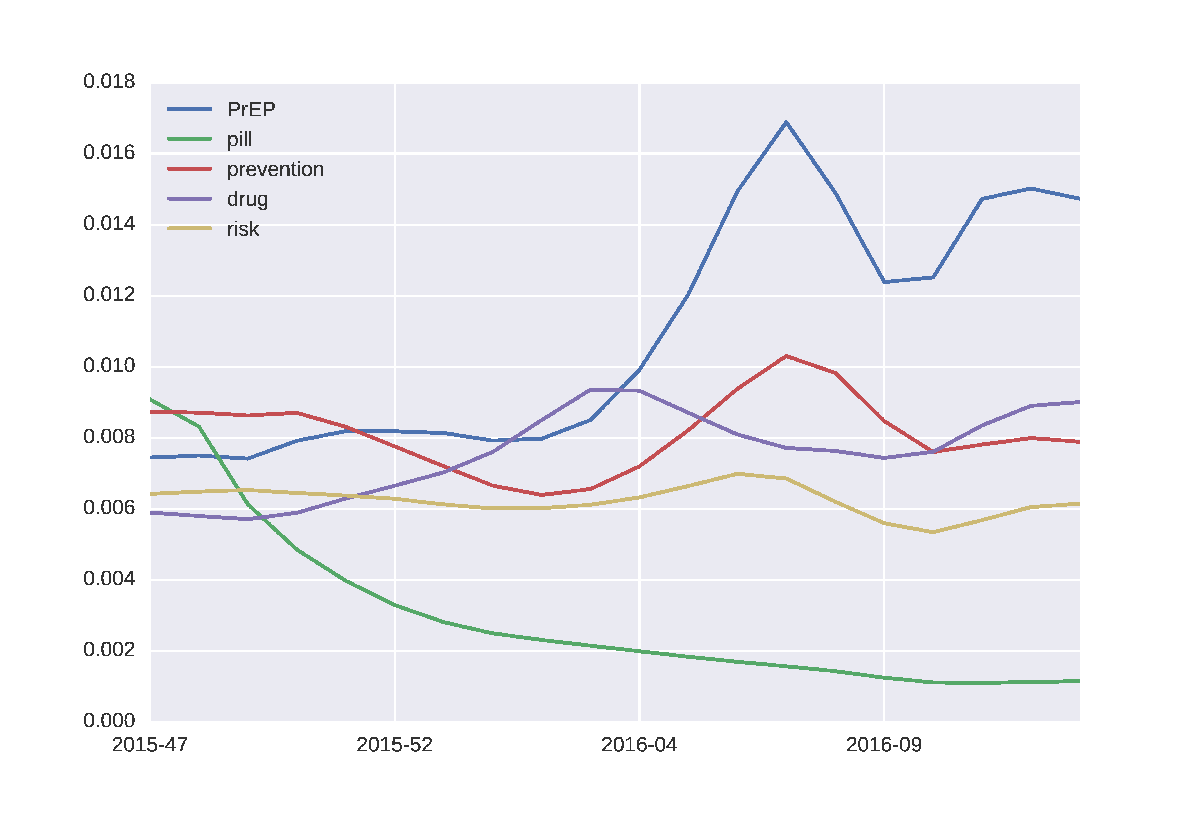
\includegraphics[height=2.5in, width=3.5in]{DTMfig1}
\caption{DTM topic 5 (PrEP related topic) word prevalence over time. Date is YYYY-WW.}
\end{figure}

We found at least one other DTM topic that showed interesting behaviour. We found that topic 4 captured several keywords related to World AIDS Day (Figure 4). We can see that 'WorldAIDSDay', and 'can' peak in the 47th week of 2015 and then decline into 2016. This correlates well with the actual date of World AIDS Day, December 1st. Furthermore, while December 1st is World AIDS day, the whole month of December is AIDS Awareness Month. We can clearly see the words 'raise' and 'awareness' peak later and last longer that the word 'WorldAIDSDay' implying that it is correlated to the whole month of December. While our PrEP investigation isn't specifically interested in World AIDS Day, or AIDS awareness month, this observation validates our ability to accurately identify temporal events using DTM. 

% figure 4
\begin{figure}
\centering
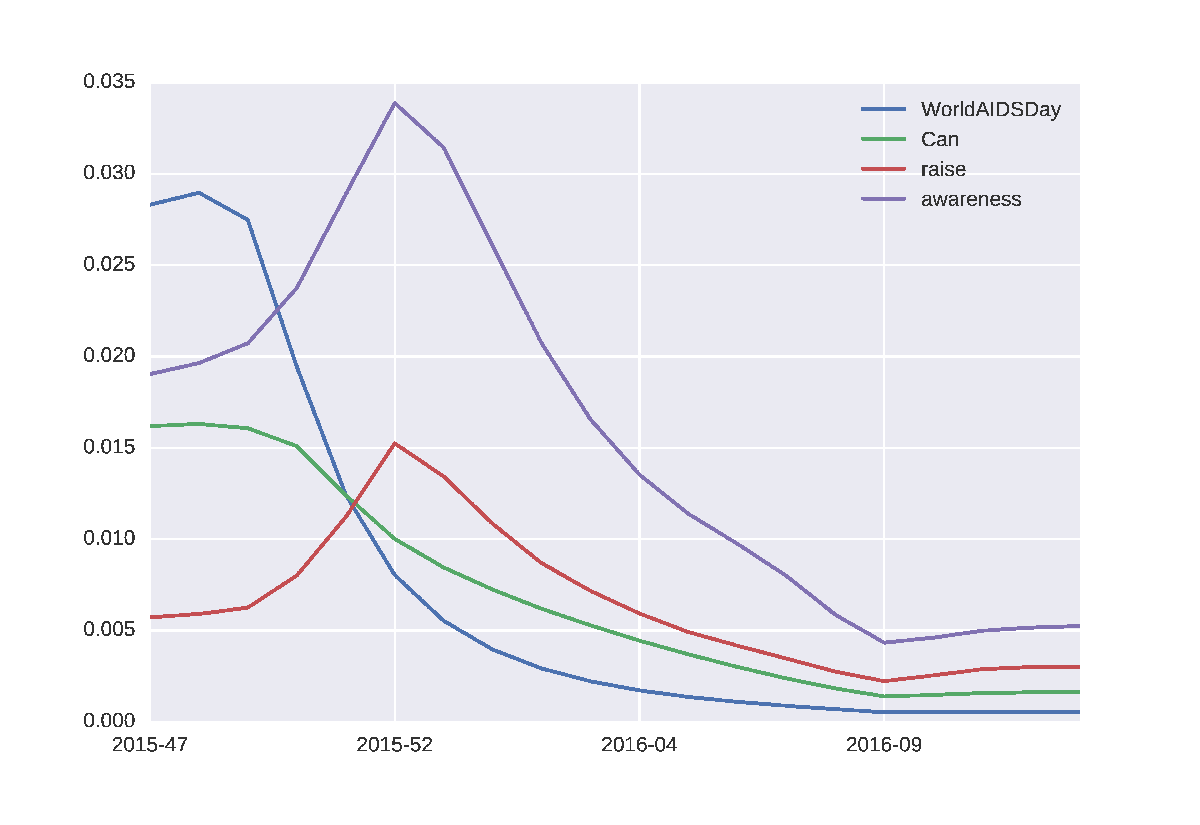
\includegraphics[height=2.5in, width=3.5in]{DTMfig2}
\caption{DTM topic 4 (WorldAIDSDay related topic) word prevalence over time. Date is YYYY-WW.}
\end{figure}

Together, the DTM results demonstrate our ability to extract relevant HIV and PrEP related information from twitter that accurately captures time-dependant fluctuations. Public health professionals should be able to monitor these temporal trends to determine the relative interest in PrEP, and other HIV related keywords as they are discussed over time. This method could even lead to a system for early detection of HIV outbreaks, or other serious developments.

\subsection{User Timeline Analysis}

% Prior to topic modelling, tweets were cleaned of high and low frequency words, and transformed by Term Frequency Inverse Document Frequency (TFIDF) processing.

% TODO work this section (re download and re-run) Tuesday

We wanted to identify what Twitter users that mentioned PrEP were discussing in their other tweets. We identified users that were most similar to PrEP according to our Paragraph2Vec results, and downloaded their most recent 3000 tweets. We took the top 400 users that had at least 200 words in the combined tweets of their tweet history. For each user, we concatenated all of their tweets, and performed LDA topic modelling on the set of user-time line documents.

When we examine a clustermap of users vs. topics, we see that the majority of these users are discussing topics 5, 1, and 4 (Figure 5). When we look up the top words in the corresponding topic distributions, we see that topics 1 and 4 seem to be related to republican party politics.

% figure 5
\begin{figure*}
\centering
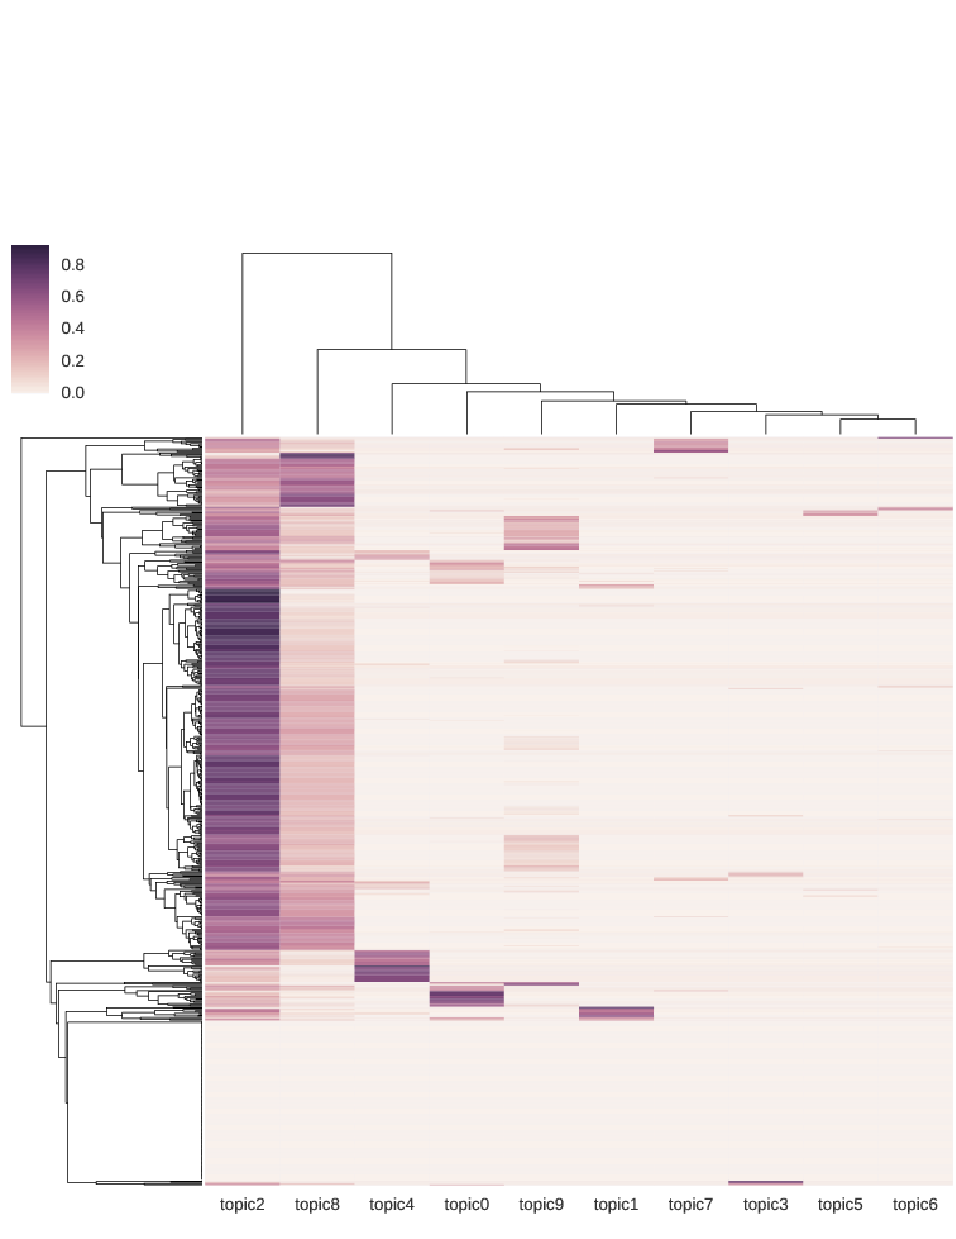
\includegraphics[height=2.5in, width=3.5in]{user_timeline_clustermap}
\caption{Clustermap of users vs. topics for the top 400 users related to PrEP.}
\end{figure*}

% table 3
\begin{table*}
\centering
\caption{Topic modeling on PrEP-related users' timelines.}
\begin{tabular}{|l|c|c|c|c|c|c|c|c|c|c|} \hline
Topic Number & Word 0 & Word 1 & Word 2 & Word 3 & Word 4 & Word 5\\ \hline
0 & wordpress & dentists & rb & aquarius & faction & reconnect\\ \hline
1 & empirefox & crooks & csr & payroll & ch & allin\\ \hline
2 & vdeo & pra & gust & lgbtqia & rail & undetectable\\ \hline
3 & hivaids & cdcstd & stigma & blacklivesmatter & realestate & getcovered\\ \hline
4 & nigga & niggas & realdonaldtrump & lmao & cruz & gop\\ \hline
5 & fertility & infertility & armenia & collage & nig & deactivate\\ \hline
6 & packaging & buenas & amigo & bu & birthcontrol & reservations \\ \hline
7 & mga & ka & socialmedia & lang & entrepreneur & naman\\ \hline
8 & infosec & bigdata & multimedia & stl & fx & malware\\ \hline
9 & nhsengland & sosa & tw & knitting & worldbank & thtorguk\\ \hline
\hline\end{tabular}
\end{table*}



Together these results suggest that PrEP users are involved in political discussions, and are internationally focused.



\subsection{Sentiment Classification}

% TODO work this section Tuesday (give example positive and negative tweets)

Lastly we trained a classifier to classify the sentiment of HIV and PrEP related tweets either positive or negative. This classifier would allow public health professionals to quickly identify positive and negative PrEP related tweets to guide HIV prevention efforts. We obtained a set of 1.6 million tweets with sentiment labels, either positive or negative from Sanders Analytics (http://www.sananalytics.com/lab/twitter-sentiment/). Then we trained a simple logistic regression classifier on 1.2 million paragraph-vectors from the sentiment dataset. We found that our classifier had an accuracy of 69\% using a portion of the sentiment tweets not used in training, as a validation set.

 We chose to use a relatively simple classifier model (logistic regression) and stop training at

We then used this classifier to classify our PrEP related tweets into positive or negative labels. We reported the most positive, and most negative tweets, by log(probability), on our full dataset, and on tweets that specifically mention either 'prep' or 'truvada' (Table 4).

% do a top positive tweets table (also with tweet ID and log prob of classification)
% table 4
\begin{table*}
\centering
\caption{Positive Sentiment Tweets.}
\begin{tabular}{|p{2cm}|p{12cm}|} \hline
Category & Text\\ \hline
General & "RT TOPublicHealth The Works provides testing for HIV anonymous \& rapid test available . Call 416-392-0520 for more info"\\ \hline
General & "RT FCAA ejaforg announced 5.4 million in grants to support orgs addressing \#HIV in new \& innovative ways!"\\ \hline
General & "RT HillaryClinton A note on the fight against HIV and AIDS and the people who really started the conversation."\\ \hline

PrEP specific & "He won't use condoms because intimacy means more than his health. but he's discovered PrEP. thank goodness."\\ \hline
PrEP specific & "PrEP Queensland Aids Council, \#HIV Foundation, Queensland."\\ \hline
PrEP specific & "RT JDatTheBody At the core of our programs is belief that young ppl can succeed in take PrEP for HIV prevention. \#NHPC2015"\\ \hline

Truvada specific & "RT CDC\_HIVAIDS Expanding testing, treatment, \& \#PrEP could prevent up to 185k new \#HIV infections"\\ \hline
Truvada specific & "Another reason 4 \#Ireland \& \#UK 2 immediately approve \#truvada \& \#PrEP 2 stop \#HIV infections . arleavitt AodhanORiordain MerchantsQuayIR"\\ \hline
Truvada specific & "RT EvanJPeterson For \#worldAIDSday my early \#PrEP arcticle in strangerslog, art by leviathanleague \#hiv \#truvada \#truvadawhore"\\ \hline

\hline\end{tabular}
\end{table*}

% do a top negative tweets table (also with tweet ID and log prob of classification)
% table 5
\begin{table*}
\centering
\caption{Negative Sentiment Tweets.}
\begin{tabular}{|p{2cm}|p{12cm}|} \hline
Category & Text\\ \hline
General & "Also, how fucking vile of Hillary to say. Reagan did fucking NOTHING during the AIDS epidemic until it was too late. What a stupid old hag."\\ \hline
General & "I wonder why he beat her ass when she was tryna leave like she wasn't gone be running back when she found out she had HIV \& nobody want her"\\ \hline
General & "Aaannd. Hillary Clinton breathes a sigh of relief that Twitter has left its outrage of her AIDS comments behind to tend to Drumpf debacle."\\ \hline

PrEP specific & "RT gaston\_croupier \#Truvada patent's not expired yet but it is sold online as a generic drug? There's something rotten in internet \#PrEP h"\\ \hline
PrEP specific & "Equality\_MI Syph \& Hep C have gone up 550\% in Gay Men bc many feel tht bc they're on PrEP, they don't need condoms. HIV isn't the only STI."\\ \hline
PrEP specific & "Xaviom8 in interviews he says he was adherent. strain was highly resistant, and Truvada wouldn't have blocked it anyways. PrEP didn't fail."\\ \hline

Truvada specific & "not surprised at all that someone got HIV on truvada. people get pregnant on birth control. tomato-condoms are still important-tomahto"\\ \hline
Truvada specific & "Now reading that truvada does not protect against certain strains of the HIV virus. Yet people want to take that risk.."\\ \hline
Truvada specific & "I think I have conjunctivitis unless truvada cured it overnight cuz im not feeling as horrible today as last night"\\ \hline

\hline\end{tabular}
\end{table*}

% there is viable information in the LDA topic modeling on positive and negative tweets

\section{Conclusions}

- Moving towards HIV outbreak prediction. 

- Automatically identifying PrEP adoption/adherence sentiment in US population.

- A lot of information on twitter is from bots, they only cost \$ per bot. This along with the character limit and slang makes twitter hard to use, but we've shown that it can be used. In fact twitter bots are slowly making twitter unusable because free advertising and marketing. Maybe in a future project we make twitter bots to spread information about PrEP.

%\end{document}  % This is where a 'short' article might terminate

%ACKNOWLEDGMENTS are optional
\section{Acknowledgments}

Acknowledgements (optional) go here.

%
% The following two commands are all you need in the
% initial runs of your .tex file to
% produce the bibliography for the citations in your paper.
\bibliographystyle{abbrv}
\bibliography{sigproc}  % sigproc.bib is the name of the Bibliography in this case
% You must have a proper ".bib" file
%  and remember to run:
% latex bibtex latex latex
% to resolve all references
%
% ACM needs 'a single self-contained file'!
%
% no appendix for now...


\subsection{References}




\end{document}
